\section{Algorytm w modelu PRAM}
\subsubsection{Algorytm sumowania}
Niech dany będzie tablica \(A\) \(n=2^k\) liczb i maszyna PRAM z n-procesorami \(\{P_1, P_2, \dots, P_n\}\). Każdy z procesorów wykonuje synchronicznie poniższy algorytm

\label{alg:crew_pram_sum}
\begin{algorithm}[H]
\SetKwFunction{Gread}{global read}
\SetKwFunction{Gwrite}{global write}
\SetKwInOut{Input}{Dane wejściowe}\SetKwInOut{Output}{Dane wyjściowe}
\Input{Tablica \(A\) długości \(n=2^k\) przechowywana w pamięci wspólnej. Każdy procesor ma zainicjalizowane zmienne lokalne \(n\) oraz identyfikator \(i\)}
\Output{Suma \(S\) wartości tablicy \(A\). Tablica \(A\) nie ulega zmianie}
\begin{enumerate}
 \item \Gread{A(i), a}
 \item \Gwrite(a, B(i))
 \item for \(h = 1\) to \( \log{n}\) do\\
	 if \(i \leq n/2^k\) then\\
	 \Gread{B(2i-1), x}\\
	 \Gread{B(2i),y}\\
	 Set z:= x + y\\
	 \Gwrite(z, B(i))\\
 \item \(if(i=1)\) then \Gwrite{z, S}
\end{enumerate}
\caption{Algorytm sumowania w PRAM\label{alg:pram_sum}}
\end{algorithm}

Przypadek dla \(n=8\) ilustruje rysunek \ref{fig:pram_sum}. W pierwszym i drugim kroku kopia B tablicy A jest tworzona w pamięci wspólnej. 
Zadania obliczeniowe w kroku 3 są na podstawie wyważonego drzewa binarnego, którego liście odpowiadają elementom tablicy A. Procesor odpowiedzialny za wykonanie za wykonanie operacji jest określony przez indeks poniżej węzła reprezentującego tę operację. Zauważmy, że procesor \(P_1\), odpowiedzialny za ustawianie wartości \(B(1)\) i zapisywanie sumy \(S\), jest zawsze aktywny w trakcie wykonywania algorytmu, podczas gdy procesory \(P_5, P_6, P_7, P_8\) są aktywne tylko podczas kroków 1 i 2.

\begin{uwaga}
Pomijamy szczegóły operacji dotyczących dostępu do pamięci. Operacje postaci \texttt{Ustaw A:=B+C}, gdzie A, B i C są zmiennymi wspólnymi będziemy interpretować jako ciąg instrukcji\\
\begin{algorithm}[H]
\SetKwFunction{Gread}{global read}
\SetKwFunction{Gwrite}{global write}
\Gread{B, x}\;
\Gread{C, y}\;
\texttt{Ustaw} z:= x + y\;
\Gwrite{z,A}\;
\end{algorithm}
\end{uwaga}

\begin{figure}[h]
\centering
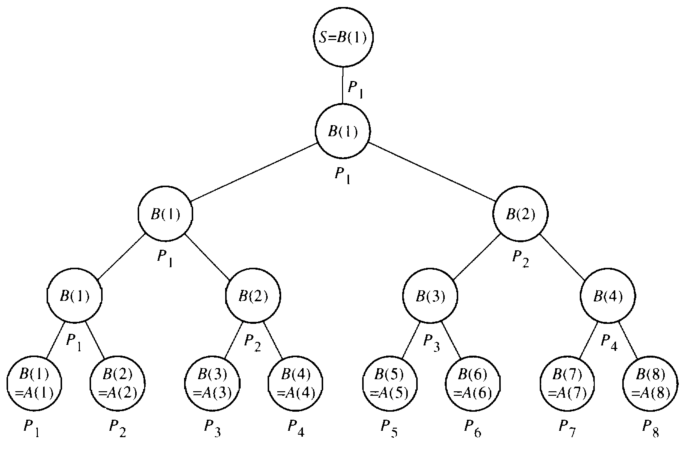
\includegraphics[width=34em]{./images/pram_sum}
\caption{Algorytm sumowania ośmiu elementów w modelu PRAM z osmioma procesorami. Każdy wewnętrzny wierzchołek grafu reprezentuje operację sumowania.}
\label{fig:pram_sum}
\end{figure}


\subsubsection{Algorytm mnożenia}
Rozważmy problem obliczenia iloczynu \(\mathbf{C}\) dwóch macierzy \(\mathbf{A}\), \(\mathbf{B}\in\mathbb{R}^{n\times n}\), gdzie \(n=2^k\), dla pewnego \(k\in\mathbf{N}\). Załóżmy, że dysponujemy \(n^3\) procesorami \(P_{i,j,l}\), \(1\leq i, j, l \leq n\) maszyny PRAM. Wówczas dla każdej pary \((i, j)\), n procesorów \(P_{i,j,l}\), gdzie \(1\leq l \leq n\), oblicza sumę \(\sum_{l=1}^{n}A(i,l)B(l,j)\) w myśl algorytmu \ref{alg:pram_sum}.\\

\label{alg:crew_pram_multiplication}
\begin{algorithm}[H]
\SetKwData{Left}{left}\SetKwData{This}{this}\SetKwData{Up}{up}
\SetKwFunction{Union}{Union}\SetKwFunction{FindCompress}{FindCompress}
\SetKwInOut{Input}{wejście}\SetKwInOut{Output}{wyjście}
\Input{Macierze \(\mathbf{A}\), \(\mathbf{B}\in\mathbb{R}^{n\times n}\), gdzie \(n=2^k\), dla pewnego \(k\in\mathbf{N}\) przechowywanych we wspólnej pamięci. Lokalnie zainicjalizowane zmienne to \(n\) i trójka wskaźników \((i, j, l)\)}
\Output{Iloczyn \(\mathbf{C=AB}\) w pamięci współdzielonej}
\begin{enumerate}
 \item \( \mathtt{Oblicz}\quad C'(i,j,l) = A(i,l)B(l,j) \)
 \item for \(h = 1\) to \( \log{n}\) do\\
 if \(l \leq n/2^k\) then \texttt{Ustaw} \(C'(i,j,l):=C'(i,j,2l-1)+C'(i,j,2l)\)
 \item \(if(l=1)\) then \texttt{Ustaw} \(C(i,j):=C'(i,j,1)\)
\end{enumerate}
\caption{Algorytm mnożenia macierzy w modelu PRAM\label{alg:pram_pseudokod}}
\end{algorithm}

\begin{uwaga}
Algorytm \ref{alg:crew_pram_multiplication} wymaga równoległego odczytu ponieważ w trakcie wykonania kroku (1) procesory \(P_{i,l,k}\) mogą równocześnie odczytywać te same dane. Przykładowo procesory \(P_{i,1,l},P_{i,2,l},\dots,P_{i,n,l}\) w trakcie wykonywania kroku (1) wszystkie wymagają dostępu do \(A(i,l)\).
\end{uwaga}

\section{Algorytmy w modelu sieciowym}
%\subsection{Jednowymiarowy torus}
%\label{alg:entorus_asynch_mesh}
%\begin{algorithm}[H]
%\SetKwInOut{Input}{Dane wejściowe}
%\SetKwInOut{Output}{Dane wyjściowe}
%\SetKwProg{ParFor}{parfor}{}{}
%\SetKwInOut{Help}{Dane pomocnicze}
%\Input{
%\begin{enumerate}
%\item podmacierze \(b=a\left((i-1)r+1\dots ir,1\dots n\right)\)
%\item \(r=\frac{n}{p}\)
%\item wektor \(x[1\dots n]\) umieszczone w procesorach \(P_i\) pracujących asynchronicznie, \(1\leq i  \leq p\) połączonych w pierścień
%\item zmienne lokalne w każdym procesorze \(P_i\) służace do przechowywania rozmiaru \(n\) oraz numeru procesora w postaci zmiennej \(i\)
%\end{enumerate}
%
%\Output{Iloczyn \(z=ax\) umieszczony w procesorze \(P_i\)}
%\Begin
%{
%\tcp*[f]{Oblczanie wektora \(y=bx\) przez procesory \(P_i, 1\leq i \leq p\)}\;
%
%\For{\(i=1 \quad \KwTo \quad n/p\)}
%{
%y[k]:=b[k,1]*x[1]\;
%\For{\(j:=1 \quad \KwTo \quad n\)}
%{
%y[k]:=y[k]+b[k,j]*x[j]\;
%}
%}
%\uIf{i:=1}{
%\(\mathtt{send}(y,prawy)\)\;
%}
%\Else{
%\(\mathtt{receive}(z[1..(i-1)r],lewy)\)\;
%\(z[1..ir]:=z[1..(i-1)]r\,||\,y\)\tcp*[f]{dopisanie wektora y}\;
%\(\mathtt{send}(z[1..ir],\,prawy)\)\;
%}
%\If{\(i=1\)}{
%\(\mathtt{receive}(z[1..n],\, lewy)\)\;
%\tcp*[f]{odebranie przez procesor \(P_1\) końcowego wyniku}\;
%}
%}
%}
%\caption{Algorytm mnożenia macierzy przez wektor w jednowymiarowym torusie}
%\end{algorithm}


\subsection{Algorytm w dwuwymiarowym torusie}
\begin{algorithm}[H]
\SetKwFunction{Prawy}{prawy}
\SetKwFunction{Dol}{dół}
\SetKwInOut{Input}{Dane wejściowe}
\SetKwInOut{Output}{Dane wyjściowe}
\SetKwProg{ParFor}{parfor}{ do}{end}
\SetKwInOut{Help}{Dane pomocnicze}
%\begin{multicols*}{2}
\Input{\begin{enumerate}
\item macierze \(a\left[1..n,\,1..n\right]\) i \(b\left[1..n,\,1..n\right]\), których elementy \(a\left[i,\,j\right]\) umieszczone są w pamięciach lokalnych procesorów \(P_{i,j}\)
\item zmienna lokalna w każdym procesorze służące do przechowyuwania rozmiaru \(n\)
\item zmienne lokalne \(i\) oraz \(j\) przechowujące numer procesora
\end{enumerate}
}

\Help{
zmienna lokalna \(k\) w każdym procesorze \(P_{i,j}\)
}
\Output{
\begin{enumerate}
\item iloczyn macierzy \(c=ab\)
\item elementy macierzy \(c[i,j]\) umieszczone w lokalnych zmiennych \(c\) procesorów \(P_{i,j}\)
\end{enumerate}
}
%\end{multicols*}
\Begin{
\For{\(k:=2\) \To \(n\)}{
\ParFor{\(P_{i,j},\, 1\leq i,\,j\leq n\) }{
\If{\(k \leq i\) }{
\(a\Longleftarrow\)\Prawy{\(a\)} \tcp*[r]{Przemieszczenie wierszy  \(a\)}
\tcp*[r]{macierzy cyklicznie w lewo}
}
\If{\(k\leq j\)}{
\(b\):=\Dol{\(b\)}\tcp*[f]{Przemieszczenie kolumn macierzy \(b\)}
\tcp*[r]{cyklicznie w górę}
}
}
}
\tcp*[h]{Obliczanie iloczynu macierzy \(a\) i \(b\)}\;
\For{\(k:=1\)\To \(n\)}{
\ParFor{\(P_{i,j}, 1\leq i,\, j\leq n\)} {
\uIf{\(k=1\)} {
c:=a*b\;
}
\Else {
a\(\Longleftarrow\)\Prawy{a}; b\(\Longleftarrow\)\Dol{b}; c:=c+a*b\;
}
}
}
}
\end{algorithm}

\subsection{Algorytm systoliczny w sieci dwuwymiarowej}

Rysunek \ref{fig:systolic_mesh} przedstawia możliwy schemat obliczenia iloczynu \(AB = C\) w myśl paradygmatu systolicznego. Wiersze macierzy \(A\) są wprowadzane synchroniczne skośnie od lewej strony sieci; kolumny macierzy \(B\) są wprowadzane synchronicznie skośnie od góry sieci.\\
Gdy procesor \(P_{i,j}\) odbierze dwie dane wejściowe \(A(i, l)\) i \(B(l,j)\), to przeprowadza operację \(C(i,j):=C(i,j+A(i,l)(B(l,j)\); po tym przesyła \(A(i,l)\) do swojego prawego sąsiada, a \(B(l,j)\) do sąsiada poniżej.

Po \(O(n)\) krokach, każdy procesor \(P_{i,j}\) będzie miał szukaną wartość \(C(i,j)\).\\

Algorytmy systoliczne pracują całkowicie synchronicznie; w każdej jednostce czasu, procesor otrzymuje dane od pewnego sąsiada, przeprowadza na nich lokalne obliczenia i następnie wysyła dane do któregoś swojego sąsiada.

\begin{figure}[h]
\centering
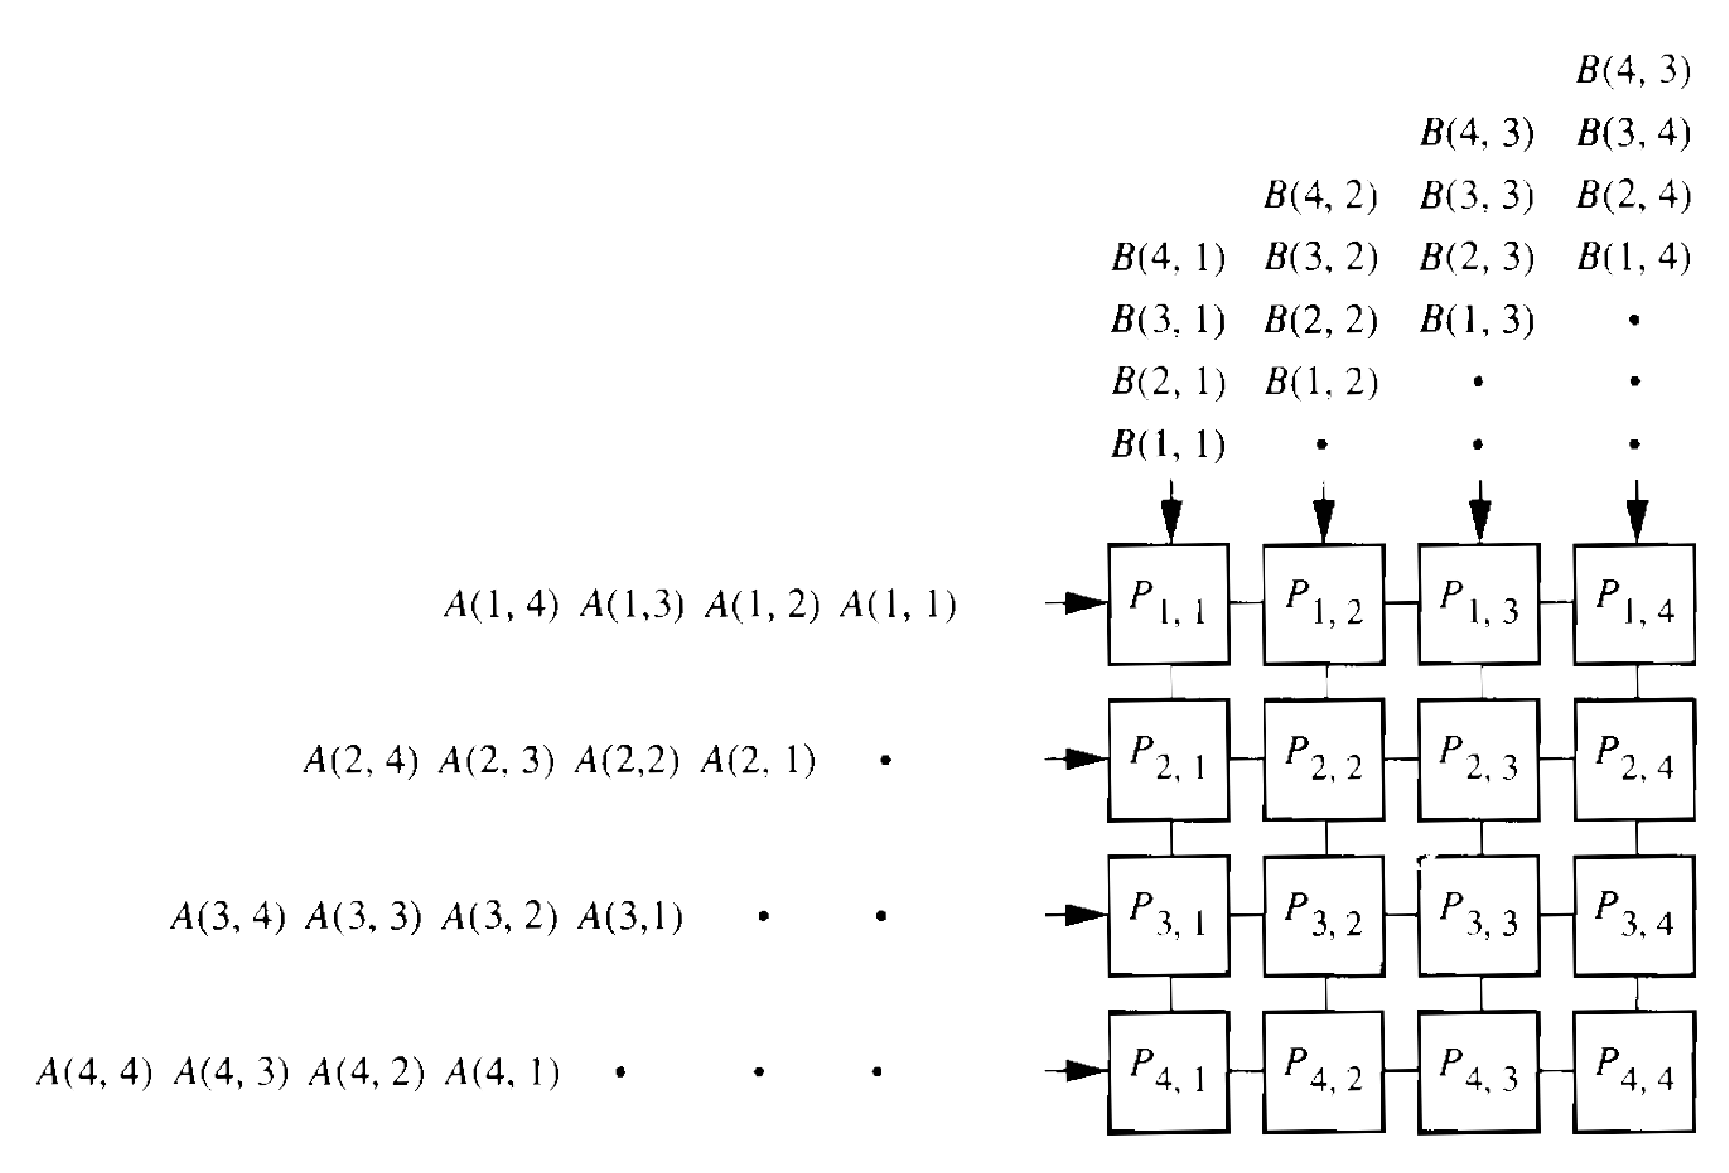
\includegraphics[width=30em]{./images/systolic2.eps}
\caption{Mnożenie macierzy w modelu sieciowym za pomocą algorytmu systolicznego. Wiersze macierzy \(\mathbf{A}\) są synchronicznie umieszczane w sieci od lewej strony, podczas, gdy równocześnie ,,od góry'' umieszczane są synchronicznie kolumny macierzy \(\mathbf{B}\). Gdy elementy \(A(i,l)\) i \(B(l,j)\) są dostępne na procesorze \(P_{i,j}\), wykonywane jest działanie \(C(i,j)=C(i,j)+A(i,l)B(l,j)\), \(A(i,l)\) zostaje wysłany do procesora \(P_{i,j+1}\) (o ile taki istnieje) oraz \(B(l,j)\) zostaje wysłany do procesora \(P_{i+1,j}\) (o ile taki istnieje).}
\label{fig:systolic_mesh}
\end{figure}

\subsection{Algorytm w topologii hipersześcianu}
\subsubsection{Rozgłaszanie ,,jednego do wszystkich'' w hipersześcianie}
Rozważmy problem rozgłaszania elementu \(X\) przechowywanego w rejestrze \(D(0)\) procesora \(P_0\) do wszystkich procesorów \(P_i\) p-procesorowego hipersześcianu, gdzie \(p=2^d\).

Algorytm polega na przechodzeniu z podkostek najniższego wymiaru, kolejno do najwyższego w \(d\) iteracjach. Pierwsza iteracja polega na wysłaniu kopii \(X\) przez procesor \(P_0\) do procesora \(P_1\). W drugiej iteracji procesor \(P_0\) i \(P_1\) wysyłają kopię \(X\) do \(P_2\) i \(P_3\) odpowiednio. Analogiczną operację przeprowadza się d-razy.




\begin{algorithm}\label{alg:broadcast_one_many}
\SetKwFunction{Prawy}{prawy}
\SetKwFunction{Dol}{dół}
\SetKwInOut{Input}{Dane wejściowe}
\SetKwInOut{Output}{Dane wyjściowe}
\SetKwProg{ParFor}{parfor}{ do}{end}
\SetKwInOut{Help}{Dane pomocnicze}
\Input{Procesor \(P_0\) z \(p=2^d\)-procesorowego synchronicznego hipersześcianu przechowuje element danych \(X\) w rejestrze \(D(0)\).}
\Output{\(X\) jest rogłaszany do wszystkich procesorów tak, że \(D(i)=X\), gdzie \(1\leq i \leq p-1\)}
\tcp*[l]{Algorytm dla procesora \(P_i\)}
\Begin{
\For{\(l=0\) \To \(d-1\)}{
\If{\(0\leq i \leq 2^l-1\)}{
Ustaw \(D(i^l):=D(i)\)\;
}
}
}
\caption{Algorytm rozgłaszania w sieci hipersześciennej}
\end{algorithm}


Algorytm \ref{alg:broadcast_one_many} ma złożoność równoległą \(\mathcal{O}(\log{p})\)

\subsubsection{Algorytm mnożenia}
Rozważmy problem mnożenia macierzy \(AB = C\) w synchronicznym hipersześcianie z \(p=n^3\) procesorów, gdzie wszystkie macierze są wymiaru \(n\times n\).\\
Niech \(n=2^q\) i stąd \(p=2^{3q}\). Przypiszmy procesorom indeksy \((l,i,j)\) takie, że \(P_{l,i,j}\) oznacza procesor \(P_r\), gdzie \(r=ln^{2}+in+j\). Innymi słowy, rozkładając indeks \(r\) binarnie otrzymuje, że \(q\) najbardziej znaczących bitów odpowiada indeksowi \(l\), następne \(q\) najbardziej znaczących bitów odpowiada indeksowi \(i\) i ostatecznie \(q\) najmniej znaczących bitow odpowiada wskaźnikowi \(j\). W szczególności, jeśli ustalimy dowolną parę wskaźników spośród \(l\), \(i\) oraz \(j\) oraz będziemy przechodzili z pozostałym wskaźnikiem po wszystkich jego możliwych wartościach, otrzymamy podkostkę wymiaru \(q\).\\

Wejściowy ciąg \(A\) jest zapamiętany w podkostce wyznaczonej przez procesory \(P_{l,i,0}\), gdzie \(0\leq l, i \leq n-1\), tak, że \(A(i,l)\) jest zapamiętane w procesorze \(P_{l,i,0}\).\\
Podobnie ciąg B jest zapamiętany w podkostce procesorów \(P_{l,0,j}\), gdzie procesor \(P_{l,0,j}\) zapamiętuje \(B(l,j)\).\\
Celem jest obliczeniem \(C(i,j)=\sum_{l=0}^{n-1}A(i,l)B(l,j)\) dla \(0\leq i, j\leq n-1\). Algorytm składa się z trzech etapów:
\begin{enumerate}
 \item Dane wejściowe są rozdystrybuowane tak, że procesor \(P_{l,i,j}\) pamięta \(A(i,l)\) i \(B(l,j)\) dla \(0\leq l, i, j \leq n-1\).
 \item Procesor \(P_{l,i,j}\) oblicza iloczyn \(C'(l,i,j)=A(i,l)B(l,j)\) dla wszystkich \(0\leq i, j, l \leq n-1\).
 \item Dla wszystkich \(0\leq i, j \leq n-1\) procesorów \(P_{l,i,j}\), gdzie \(0\leq l\leq n-1\), obliczają sumę \(C(i,j)=\sum_{i=0}^{n-1} C'(l,i,j)\)
\end{enumerate}

Implementacja pierwszego etapu składa się z dwóch części. W pierwszej z nich \emph{rozgłaszamy}, dla każdego \(i, l, A(i,l)\), z procesora \(P_{i,l,0}\) do \(P_{l,i,})\) dla \(0\leq j \leq n-1\). Ponieważ zbiór procesorów \(\{P_{l,i,j}|0\leq j \leq n-1\}\) wyznacza q-wymiarową kostkę dla każdej z par \(i\) oraz \(l\), możemy użyć \textbf{algorytmu rozgłaszania}, żeby rozgłosić \(A(i,l)\) od procesora \(P_{l,i,0}\) do wszystkich procesorów \(P_{l,i,j}\).
W drugiej części każdy element \(B(l,j)\) przechowywany w procesorze \(P_{l,0,j}\) jest rozgłaszany do procesorów \(P_{l,i,j}\) dla wszystkich \(0\leq i \leq n-1\). Pod koniec procesor \(P_{l,i,j}\) będzie przechowywał dwie wartości: \(A(i,l)\) i \(B(l,j)\). Używając algorytmu (tutaj referencja) etap pierwszy ma równoległą złożonośc czasową \(O(\log{n})\).

Drugi etap polega na wykonywaniu pojedyńczych mnożeń na każdym z procesorów \(P_{l,i,j}\). Stąd etap na etap ten składa się tylko jeden równoległy krok obliczeniowy. Pod koniec procesor \(P_{l,i,j}\) przechowuje \(C'(l,i,j)\).

Trzeci etap polega na obliczeniu \(n^2\) sum \(C(i,j)\). Wartości \(C'(l,i,j)\) każdej z sum znajudują się w q-wymiarowym hipersześcianie \(\{P_{l,i,j}\,|\,0\leq l\leq n-1\}\). Obliczanie takich sum ma równoległą złożoność czasową \(O(\log{n}\). Procesor \(P_{0,i,j}\) będzie przechowywał wartość \(C(i,j)\) iloczynu.

Wobec powyższych iloczyn macierzy wymiaru \(n \times n\) w sieci hipersześciennej może być obliczony w czasie \(O(\log{n})\) dysponując \(n^3\) procesorami.
\subsection{Algorytm Cannona w dwuwymiarowej sieci}
\cite{communication_efficient}
\subsection{Algorytm 2.5D}
\cite{Solomonik:EECS-2011-72}
\subsection{Algorytm 3D}
\cite{communication_efficient}
\subsection{Równoległy algorytm Strassena CAPS}
\cite{DBLP:journals/corr/abs-1202-3173}